\documentclass[12pt]{article}

\usepackage{amsmath}
\usepackage{amsfonts}
\usepackage[affil-it]{authblk}
\usepackage{listings}
\usepackage{float}
\usepackage{fancyhdr}
\usepackage{graphicx}
\usepackage[colorlinks=true,linkcolor=blue, citecolor=red]{hyperref}
\usepackage{url}
\usepackage[top=.75in, left=.5in, right=.5in, bottom=1in]{geometry}
\usepackage[utf8]{vietnam}
\usepackage{xcolor}
\setlength{\headheight}{29.43912pt}

% \graphicspath{PATH_TO_GRAPHIC_FOLDER}


\definecolor{codegreen}{rgb}{0,0.6,0}
\definecolor{codegray}{rgb}{0.5,0.5,0.5}
\definecolor{codepurple}{rgb}{0.58,0,0.82}
\definecolor{backcolour}{rgb}{0.95,0.95,0.92}

\lstdefinestyle{mystyle}{
    backgroundcolor=\color{backcolour},   
    commentstyle=\color{codegreen},
    keywordstyle=\color{magenta},
    numberstyle=\tiny\color{codegray},
    stringstyle=\color{codepurple},
    basicstyle=\ttfamily\footnotesize,
    breakatwhitespace=false,         
    breaklines=true,                 
    captionpos=b,                    
    keepspaces=true,                 
    numbers=left,                    
    numbersep=5pt,                  
    showspaces=false,                
    showstringspaces=false,
    showtabs=false,                  
    tabsize=2
}

\lstset{style=mystyle}

\newcommand{\coursename}{CSC10104 - Quy hoạch tuyến tính}
\newcommand{\reportname}{Một ví dụ cho bài toán Klee-Minty với $n = 4$}

\pagestyle{fancy}
\lhead{
\reportname
}
\rhead{
Trường Đại học Khoa học Tự nhiên - ĐHQG HCM\\
\coursename
}
\lfoot{\LaTeX\ by \href{https://github.com/trhgquan}{Quan, Tran Hoang}}

\title{\textbf{\reportname}}
\author{Trần Hoàng Quân%
  \thanks{MSSV: 19120338;}}
\affil{Trường Đại học Khoa học Tự nhiên, ĐHQG-HCM}

\author{Đoàn Thu Ngân%
  \thanks{MSSV: 19120xxx;}}
\affil{Trường Đại học Khoa học Tự nhiên, ĐHQG-HCM}

\begin{document}
\maketitle

\begin{abstract}
Trong bài này, nhóm nhắc lại định nghĩa về Bài toán Klee-Minty \ref{klee-minty-revised}. Để đưa ra một ví dụ minh họa, nhóm chọn Bài tập 4.5 từ quyển Linear Programming của tác giả Robert J. Vanderbei \ref{Vanderbei-4.5}. Qua đó, nhóm đưa ra kết luận rằng bài toán Klee-Minty cần ít nhất $2^n - 1$ lần lặp để tìm ra được phương án tối ưu, với $n$ là số ràng buộc và số biến.
\end{abstract}

\section{Nhắc lại bài toán Klee-Minty}\label{klee-minty-revised}
Bài toán Klee-Minty là một bài toán quy hoạch tuyến tính có $n$ ràng buộc và $n$ biến, được đưa ra bởi V.Klee và G.J. Minty vào năm 1972\cite{Vanderbei2020}. Theo đó, để giải bài toán này dùng Phương pháp đơn hình cần ít nhất $2^{n} - 1$ lần lặp (hay nói cách khác, cần lập $2^{n} - 1$ bảng đơn hình để tìm ra phương án tối ưu). Bài toán được phát biểu như sau:\\\\
Hàm mục tiêu
$$
f(x_1, .., x_n) = \sum_{j = 1}^n 2^{n - j}x_j \rightarrow \max
$$
các ràng buộc
\begin{equation*}
\begin{aligned}
2\sum_{j = 1}^{i - 1} 2^{i - j}x_j + x_i &\leq 100^{i - 1}\ &i = \overline{1, n}\\
x_j &\geq 0\ &j = \overline{1, n}
\end{aligned}
\end{equation*}
Tổng quát hóa: đặt $\beta_i = 100^{i - 1}$. Khi đó dạng tổng quát hóa của Bài toán Klee-Minty trở thành:\\\\
Hàm mục tiêu
$$
\sum_{j = 1}^n 2^{n - j}x_j - \frac{1}{2}\sum_{j = 1}^{n} 2^{n - j}\beta_j \rightarrow \max
$$
các ràng buộc
\begin{equation*}
\begin{aligned}
\sum_{j = 1}^{i - 1} 2^{i - j} x_j + x_i &\leq \sum_{j = 1}^{i - 1} 2^{i - j} \beta_j + \beta_i\ &i = \overline{1, n}\\
x_j &\leq 0\ &j = \overline{1, n}
\end{aligned}
\end{equation*}
Bài toán Klee-Minty là ví dụ cho trường hợp xấu nhất của Phương pháp đơn hình, khi đó ta tốn nhiều chi phí tính toán nhất để giải quyết một bài toán.

\section{Bài tập 4.5 sách Vanderbei}\label{Vanderbei-4.5}
\subsection{Đề bài}
Giải bài toán Klee-Minty 4 biến. Chi tiết hơn, với trường hợp $n = 4$, hàm mục tiêu trở thành
$$
f(x_1, x_2, x_3, x_4) = 8x_1 + 4x_2 + 2x_3 + x_4 - 4\beta_1 - 2\beta_2 - \beta_3 - \frac{1}{2}\beta_4 \rightarrow \max
$$
các ràng buộc
$$
\left\{
\begin{array}{lll}
x_1 &\leq \beta_1 \\
4x_1 + x_2 &\leq 2\beta_1 + \beta_2 \\
8x_1 + 4x_2 + x_3 &\leq 4\beta_1 + 2\beta_2 + \beta_3 \\
16x_1 + 8x_2 + 4x_3 + x_4 &\leq 8\beta_1 + 4\beta_2 + 2\beta_3 + \beta_4 \\
x_j &\geq 0\ &j = \overline{1, 4}
\end{array}
\right.
$$

\subsection{Lời giải - phương pháp đơn hình}
Bổ sung các biến $x_5, x_6, x_7, x_8$ để biến hệ ràng buộc bất đẳng thức về dạng đẳng thức:
$$
\left\{
\begin{array}{lll}
x_1 + x_5 &= \beta_1 \\
4x_1 + x_2 + x_6 &= 2\beta_1 + \beta_2 \\
8x_1 + 4x_2 + x_3 + x_7 &= 4\beta_1 + 2\beta_2 + \beta_3 \\
16x_1 + 8x_2 + 4x_3 + x_4 + x_8 &= 8\beta_1 + 4\beta_2 + 2\beta_3 + \beta_4 \\
x_j &\geq 0\ &j = \overline{1, 4}
\end{array}
\right.
$$
Bảng đơn hình xuất phát như sau:
\begin{table}[H]
\centering
\begin{tabular}{|c|c|c|c|c|c|c|c|c|c|c|}
\hline
CS & HS & PA & 8 & 4 & 2 & 1 & 0 & 0 & 0 & 0 \\
\hline
$x_5$ & 0 & $\beta_1$ & 1 & 0 & 0 & 0 & 1 & 0 & 0 & 0 \\
$x_6$ & 0 & $2\beta_1 + \beta_2$ & 4 & 1 & 0 & 0 & 0 & 1 & 0 & 0 \\
$x_7$ & 0 & $4\beta_1 + 2\beta_2 + \beta_3$ & 8 & 4 & 1 & 0 & 0 & 0 & 1 & 0 \\
$x_8$ & 0 & $8\beta_1 + 4\beta_2 + 2\beta_3 + \beta_4$ & 16 & 8 & 4 & 1 & 0 & 0 & 0 & 1 \\
\hline
\multicolumn{2}{|c|}{$f_{\max}$}
& 0 & -8 & -4 & -2 & -1 & 0 & 0 & 0 & 0 \\
\hline
\end{tabular}
\end{table}

\subsubsection{Lần lặp thứ 1}
\begin{itemize}
\item Nhận thấy có 4 cột có $\Delta < 0$, ta chọn cột có $\Delta = -8$.
\item Xét tỷ lệ $\displaystyle \frac{\beta_1}{1} < \frac{2\beta_1 + \beta_2}{4} < \frac{4\beta_1 + 2\beta_2 + \beta_3}{8} < \frac{8\beta_1 + 4\beta_2 + 2\beta_3 + \beta_4}{16}$, nên ta chọn dòng 1.
\item Khi đó $x_5$ ra, $x_1$ vào.
\end{itemize}
Tiến hành biến đổi:
$$
\left\{
\begin{array}{lll}
d_1 \leftarrow d_1 \\
d_2 \leftarrow d_2 - 4d_1 \\
d_3 \leftarrow d_3 - 8d_1 \\
d_4 \leftarrow d_4 - 16d_1 \\
\end{array}
\right.
$$
Bảng đơn hình cho lần lặp đầu tiên như sau:
\begin{table}[H]
\centering
\begin{tabular}{|c|c|c|c|c|c|c|c|c|c|c|}
\hline
CS & HS & PA & 8 & 4 & 2 & 1 & 0 & 0 & 0 & 0 \\
\hline
$x_1$ & 8 & $\beta_1$ & 1 & 0 & 0 & 0 & 1 & 0 & 0 & 0 \\
$x_6$ & 0 & $-2\beta_1 + \beta_2$ & 0 & 1 & 0 & 0 & -4 & 1 & 0 & 0 \\
$x_7$ & 0 & $-4\beta_1 + 2\beta_2 + \beta_3$ & 0 & 4 & 1 & 0 & -8 & 0 & 1 & 0 \\
$x_8$ & 0 & $-8\beta_1 + 4\beta_2 + 2\beta_3 + \beta_4$ & 0 & 8 & 4 & 1 & -16 & 0 & 0 & 1 \\
\hline
\multicolumn{2}{|c|}{$f_{\max}$}
& $8\beta_1$ & 0 & -4 & -2 & -1 & 8 & 0 & 0 & 0 \\
\hline
\end{tabular}
\end{table}

\subsubsection{Lần lặp thứ 2}
\begin{itemize}
\item Tồn tại 3 cột có $\Delta < 0$, ta chọn cột có $\Delta = -4$.
\item Xét tỷ lệ $\displaystyle \frac{-2\beta_1 + \beta_2}{1} < \frac{-4\beta_1 + 2\beta_2 + \beta_3}{4} < \frac{-8\beta_1 + 4\beta_2 + 2\beta_3 + \beta_4}{8}$, nên ta chọn dòng 2.
\item Vậy $x_6$ ra, $x_2$ vào.
\end{itemize}
Tiến hành biến đổi:
$$
\left\{
\begin{array}{lll}
d_1 \leftarrow d_1 \\
d_2 \leftarrow d_2 \\
d_3 \leftarrow d_3 - 4d_2 \\
d_4 \leftarrow d_4 - 8d_2
\end{array}
\right.
$$
Bảng đơn hình cho lần lặp thứ 2 như sau:
\begin{table}[H]
\centering
\begin{tabular}{|c|c|c|c|c|c|c|c|c|c|c|}
\hline
CS & HS & PA & 8 & 4 & 2 & 1 & 0 & 0 & 0 & 0 \\
\hline
$x_1$ & 8 & $\beta_1$ & 1 & 0 & 0 & 0 & 1 & 0 & 0 & 0 \\
$x_2$ & 4 & $-2\beta_1 + \beta_2$ & 0 & 1 & 0 & 0 & -4 & 1 & 0 & 0 \\
$x_7$ & 0 & $4\beta_1 - 2\beta_2 + \beta_3$ & 0 & 0 & 1 & 0 & 8 & -4 & 1 & 0 \\
$x_8$ & 0 & $8\beta_1 - 4\beta_2 + 2\beta_3 + \beta_4$ & 0 & 0 & 4 & 1 & 16 & -8 & 0 & 1 \\
\hline
\multicolumn{2}{|c|}{$f_{\max}$}
& $4\beta_2$ & 0 & 0 & -2 & -1 & -8 & 4 & 0 & 0 \\
\hline
\end{tabular}
\end{table}

\subsubsection{Lần lặp thứ 3}
\begin{itemize}
\item Tồn tại 3 cột có $\Delta < 0$, ta chọn cột có $\Delta = -8$.
\item Tỷ lệ $\displaystyle \frac{\beta_1}{1} < \frac{4\beta_1 - 2\beta_2 + \beta_3}{8} < \frac{8\beta_1 - 4\beta_2 + 2\beta_3 + \beta_4}{16}$ nên ta chọn dòng 1.
\item Vậy $x_1$ ra, $x_5$ vào.
\end{itemize}
Tiến hành biến đổi:
$$
\left\{
\begin{array}{lll}
d_1 \leftarrow d_1 \\
d_2 \leftarrow d_2 + 4d_1 \\
d_3 \leftarrow d_3 - 8d_1 \\
d_4 \leftarrow d_4 - 16d_1
\end{array}
\right.
$$
Bảng đơn hình cho lần lặp thứ 3 như sau:
\begin{table}[H]
\centering
\begin{tabular}{|c|c|c|c|c|c|c|c|c|c|c|}
\hline
CS & HS & PA & 8 & 4 & 2 & 1 & 0 & 0 & 0 & 0 \\
\hline
$x_5$ & 0 & $\beta_1$ & 1 & 0 & 0 & 0 & 1 & 0 & 0 & 0 \\
$x_2$ & 4 & $2\beta_1 + \beta_2$ & 4 & 1 & 0 & 0 & 0 & 1 & 0 & 0 \\
$x_7$ & 0 & $-4\beta_1 - 2\beta_2 + \beta_3$ & -8 & 0 & 1 & 0 & 0 & -4 & 1 & 0 \\
$x_8$ & 0 & $-8\beta_1 - 4\beta_2 + 2\beta_3 + \beta_4$ & -16 & 0 & 4 & 1 & 0 & 8 & 0 & 1 \\
\hline
\multicolumn{2}{|c|}{$f_{\max}$}
& $8\beta_1 + 4\beta_2$ & 8 & 0 & -2 & -1 & 0 & 4 & 0 & 0 \\
\hline
\end{tabular}
\end{table}

\subsubsection{Lần lặp thứ 4}
\begin{itemize}
\item Tồn tại 2 cột có $\Delta < 0$, ta chọn cột có $\Delta = -2$.
\item Tỷ lệ $\displaystyle \frac{-4\beta_1 - 2\beta_2 + \beta_3}{1} < \frac{-8\beta_1 - 4\beta_2 + 2\beta_3 + \beta_4}{4}$ nên ta chọn dòng 3.
\item Vậy $x_7$ ra, $x_3$ vào.
\end{itemize}
Tiến hành biến đổi:
$$
\left\{
\begin{array}{lll}
d_1 \leftarrow d_1 \\
d_2 \leftarrow d_2 \\
d_3 \leftarrow d_3\\
d_4 \leftarrow d_4 - 4d_3
\end{array}
\right.
$$
Bảng đơn hình cho lần lặp thứ 4 như sau:
\begin{table}[H]
\centering
\begin{tabular}{|c|c|c|c|c|c|c|c|c|c|c|}
\hline
CS & HS & PA & 8 & 4 & 2 & 1 & 0 & 0 & 0 & 0 \\
\hline
$x_5$ & 0 & $\beta_1$ & 1 & 0 & 0 & 0 & 1 & 0 & 0 & 0 \\
$x_2$ & 4 & $2\beta_1 + \beta_2$ & 4 & 1 & 0 & 0 & 0 & 1 & 0 & 0 \\
$x_3$ & 2 & $-4\beta_1 - 2\beta_2 + \beta_3$ & -8 & 0 & 1 & 0 & 0 & -4 & 1 & 0 \\
$x_8$ & 0 & $8\beta_1 + 4\beta_2 - 2\beta_3 + \beta_4$ & 16 & 0 & 0 & 1 & 0 & 8 & -4 & 1 \\
\hline
\multicolumn{2}{|c|}{$f_{\max}$}
& $2\beta_3$ & -8 & 0 & 0 & 0 & 0 & -4 & 2 & 0 \\
\hline
\end{tabular}
\end{table}

\subsubsection{Lần lặp thứ 5}
\begin{itemize}
\item Tồn tại 2 cột có $\Delta < 0$, ta chọn cột có $\Delta = -8$.
\item Tỷ lệ $\displaystyle \frac{\beta_1}{1} < \frac{2\beta_1 + \beta_2}{4} < \frac{8\beta_1 + 4\beta_2 - 2\beta_3 + \beta_4}{16}$ nên ta chọn dòng 1.
\item Vậy $x_5$ ra, $x_1$ vào.
\end{itemize}
Tiến hành biến đổi:
$$
\left\{
\begin{array}{lll}
d_1 \leftarrow d_1 \\
d_2 \leftarrow d_2 - 4d_1 \\
d_3 \leftarrow d_3 + 8d_1\\
d_4 \leftarrow d_4 - 16d_1
\end{array}
\right.
$$
Bảng đơn hình cho lần lặp thứ 5 như sau:
\begin{table}[H]
\centering
\begin{tabular}{|c|c|c|c|c|c|c|c|c|c|c|}
\hline
CS & HS & PA & 8 & 4 & 2 & 1 & 0 & 0 & 0 & 0 \\
\hline
$x_1$ & 8 & $\beta_1$ & 1 & 0 & 0 & 0 & 1 & 0 & 0 & 0 \\
$x_2$ & 4 & $-2\beta_1 + \beta_2$ & 0 & 1 & 0 & 0 & -4 & 1 & 0 & 0 \\
$x_3$ & 2 & $4\beta_1 - 2\beta_2 + \beta_3$ & 0 & 0 & 1 & 0 & 8 & -4 & 1 & 0 \\
$x_8$ & 0 & $-8\beta_1 + 4\beta_2 - 2\beta_3 + \beta_4$ & 0 & 0 & 0 & 1 & -16 & 8 & -4 & 1 \\
\hline
\multicolumn{2}{|c|}{$f_{\max}$}
& $8\beta_1 + 2\beta_3$ & 0 & 0 & 0 & 0 & 8 & -4 & 2 & 0 \\
\hline
\end{tabular}
\end{table}

\subsubsection{Lần lặp thứ 6}
\begin{itemize}
\item Tồn tại 1 cột có $\Delta < 0$, ta chọn cột có $\Delta = -4$.
\item Tỷ lệ $\displaystyle \frac{-2\beta_1 + \beta_2}{1} < \frac{-8\beta_1 + 4\beta_2 - 2\beta_3 + \beta_4}{8}$ nên ta chọn dòng 2.
\item Vậy $x_2$ ra, $x_6$ vào.
\end{itemize}
Tiến hành biến đổi:
$$
\left\{
\begin{array}{lll}
d_1 \leftarrow d_1 \\
d_2 \leftarrow d_2 \\
d_3 \leftarrow d_3 + 4d_2\\
d_4 \leftarrow d_4 - 8d_2
\end{array}
\right.
$$
Bảng đơn hình cho lần lặp thứ 6 như sau:
\begin{table}[H]
\centering
\begin{tabular}{|c|c|c|c|c|c|c|c|c|c|c|}
\hline
CS & HS & PA & 8 & 4 & 2 & 1 & 0 & 0 & 0 & 0 \\
\hline
$x_1$ & 8 & $\beta_1$ & 1 & 0 & 0 & 0 & 1 & 0 & 0 & 0 \\
$x_6$ & 0 & $-2\beta_1 + \beta_2$ & 0 & 1 & 0 & 0 & -4 & 1 & 0 & 0 \\
$x_3$ & 2 & $-4\beta_1 + 2\beta_2 + \beta_3$ & 0 & 4 & 1 & 0 & -8 & 0 & 1 & 0 \\
$x_8$ & 0 & $8\beta_1 - 4\beta_2 - 2\beta_3 + \beta_4$ & 0 & -8 & 0 & 1 & 16 & 0 & -4 & 1 \\
\hline
\multicolumn{2}{|c|}{$f_{\max}$}
& $4\beta_2 + 2\beta_3$ & 0 & 4 & 0 & 0 & -8 & 0 & 2 & 0 \\
\hline
\end{tabular}
\end{table}

\subsubsection{Lần lặp thứ 7}
\begin{itemize}
\item Tồn tại 1 cột có $\Delta < 0$, ta chọn cột có $\Delta = -8$.
\item Chỉ có 1 dòng $d_1$ có tỷ số $\displaystyle \frac{\beta_1}{1} > 0$, nên ta chọn dòng 1.
\item Vậy $x_1$ ra, $x_5$ vào.
\end{itemize}
Tiến hành biến đổi:
$$
\left\{
\begin{array}{lll}
d_1 \leftarrow d_1 \\
d_2 \leftarrow d_2 + 4d_1 \\
d_3 \leftarrow d_3 + 8d_1\\
d_4 \leftarrow d_4 - 16d_1
\end{array}
\right.
$$
Bảng đơn hình cho lần lặp thứ 7 như sau:
\begin{table}[H]
\centering
\begin{tabular}{|c|c|c|c|c|c|c|c|c|c|c|}
\hline
CS & HS & PA & 8 & 4 & 2 & 1 & 0 & 0 & 0 & 0 \\
\hline
$x_5$ & 0 & $\beta_1$ & 1 & 0 & 0 & 0 & 1 & 0 & 0 & 0 \\
$x_6$ & 0 & $2\beta_1 + \beta_2$ & 4 & 1 & 0 & 0 & 0 & 1 & 0 & 0 \\
$x_3$ & 2 & $4\beta_1 + 2\beta_2 + \beta_3$ & 8 & 4 & 1 & 0 & 0 & 0 & 1 & 0 \\
$x_8$ & 0 & $-8\beta_1 - 4\beta_2 - 2\beta_3 + \beta_4$ & -16 & -8 & 0 & 1 & 0 & 0 & -4 & 1 \\
\hline
\multicolumn{2}{|c|}{$f_{\max}$}
& $8\beta_1 + 4\beta_2 + 2\beta_3$ & 8 & 4 & 0 & -1 & 0 & 0 & 2 & 0 \\
\hline
\end{tabular}
\end{table}

\subsubsection{Lần lặp thứ 8}
\begin{itemize}
\item Tồn tại 1 cột có $\Delta < 0$, ta chọn cột có $\Delta = -1$.
\item Chỉ có 1 dòng $d_4$ có tỷ số $\displaystyle \frac{24\beta_1 - 4\beta_2 - 2\beta_3 + \beta_4}{1} > 0$, nên ta chọn dòng 4.
\item Vậy $x_8$ ra, $x_4$ vào.
\end{itemize}
Tiến hành biến đổi:
$$
\left\{
\begin{array}{lll}
d_1 \leftarrow d_1 \\
d_2 \leftarrow d_2\\
d_3 \leftarrow d_3\\
d_4 \leftarrow d_4 + 4d_1
\end{array}
\right.
$$
Bảng đơn hình cho lần lặp thứ 8 như sau:
\begin{table}[H]
\centering
\begin{tabular}{|c|c|c|c|c|c|c|c|c|c|c|}
\hline
CS & HS & PA & 8 & 4 & 2 & 1 & 0 & 0 & 0 & 0 \\
\hline
$x_5$ & 0 & $\beta_1$ & 1 & 0 & 0 & 0 & 1 & 0 & 0 & 0 \\
$x_6$ & 0 & $2\beta_1 + \beta_2$ & 4 & 1 & 0 & 0 & 0 & 1 & 0 & 0 \\
$x_3$ & 2 & $4\beta_1 + 2\beta_2 + \beta_3$ & 8 & 4 & 1 & 0 & 0 & 0 & 1 & 0 \\
$x_4$ & 1 & $-8\beta_1 - 4\beta_2 - 2\beta_3 + \beta_4$ & -16 & -8 & 0 & 1 & 0 & 0 & -4 & 1 \\
\hline
\multicolumn{2}{|c|}{$f_{\max}$}
& $\beta_4$ & -8 & -4 & 0 & 0 & 0 & 0 & -2 & 1 \\
\hline
\end{tabular}
\end{table}

\subsubsection{Lần lặp thứ 9}
\begin{itemize}
\item Tồn tại 3 cột có $\Delta < 0$, ta chọn cột có $\Delta = -8$.
\item Xét tỷ số $\displaystyle \frac{\beta_1}{1} < \frac{2\beta_1 + \beta_2}{4} < \frac{4\beta_1 + 2\beta_2 + \beta_3}{8}$, nên ta chọn dòng 1.
\item Vậy $x_5$ ra, $x_1$ vào.
\end{itemize}
Tiến hành biến đổi:
$$
\left\{
\begin{array}{lll}
d_1 \leftarrow d_1 \\
d_2 \leftarrow d_2 - 4d_1\\
d_3 \leftarrow d_3 - 8d_1\\
d_4 \leftarrow d_4 + 16d_1
\end{array}
\right.
$$
Bảng đơn hình cho lần lặp thứ 9 như sau:
\begin{table}[H]
\centering
\begin{tabular}{|c|c|c|c|c|c|c|c|c|c|c|}
\hline
CS & HS & PA & 8 & 4 & 2 & 1 & 0 & 0 & 0 & 0 \\
\hline
$x_1$ & 8 & $\beta_1$ & 1 & 0 & 0 & 0 & 1 & 0 & 0 & 0 \\
$x_6$ & 0 & $-2\beta_1 + \beta_2$ & 0 & 1 & 0 & 0 & -4 & 1 & 0 & 0 \\
$x_3$ & 2 & $-4\beta_1 + 2\beta_2 + \beta_3$ & 0 & 4 & 1 & 0 & -8 & 0 & 1 & 0 \\
$x_4$ & 1 & $8\beta_1 - 4\beta_2 - 2\beta_3 + \beta_4$ & 0 & -8 & 0 & 1 & 16 & 0 & -4 & 1 \\
\hline
\multicolumn{2}{|c|}{$f_{\max}$}
& $8\beta_1 + \beta_4$ & 0 & -4 & 0 & 0 & 8 & 0 & -2 & 1 \\
\hline
\end{tabular}
\end{table}

\subsubsection{Lần lặp thứ 10}
\begin{itemize}
\item Tồn tại 2 cột có $\Delta < 0$, ta chọn cột có $\Delta = -4$.
\item Xét tỷ số $\displaystyle \frac{-2\beta_1 + \beta_2}{1} < \frac{-4\beta_1 + 2\beta_2 + \beta_3}{4}$, nên ta chọn dòng 2.
\item Vậy $x_6$ ra, $x_2$ vào.
\end{itemize}
Tiến hành biến đổi:
$$
\left\{
\begin{array}{lll}
d_1 \leftarrow d_1 \\
d_2 \leftarrow d_2\\
d_3 \leftarrow d_3 - 4d_2\\
d_4 \leftarrow d_4 + 8d_2
\end{array}
\right.
$$
Bảng đơn hình cho lần lặp thứ 10 như sau:
\begin{table}[H]
\centering
\begin{tabular}{|c|c|c|c|c|c|c|c|c|c|c|}
\hline
CS & HS & PA & 8 & 4 & 2 & 1 & 0 & 0 & 0 & 0 \\
\hline
$x_1$ & 8 & $\beta_1$ & 1 & 0 & 0 & 0 & 1 & 0 & 0 & 0 \\
$x_2$ & 4 & $-2\beta_1 + \beta_2$ & 0 & 1 & 0 & 0 & -4 & 1 & 0 & 0 \\
$x_3$ & 2 & $4\beta_1 - 2\beta_2 + \beta_3$ & 0 & 0 & 1 & 0 & 8 & -4 & 1 & 0 \\
$x_4$ & 1 & $-8\beta_1 + 4\beta_2 - 2\beta_3 + \beta_4$ & 0 & 0 & 0 & 1 & -16 & 8 & -4 & 1 \\
\hline
\multicolumn{2}{|c|}{$f_{\max}$}
& $4\beta_2 + \beta_4$ & 0 & 0 & 0 & 0 & -16 & 4 & -2 & 1 \\
\hline
\end{tabular}
\end{table}

\subsubsection{Lần lặp thứ 11}
\begin{itemize}
\item Tồn tại 2 cột có $\Delta < 0$, ta chọn cột có $\Delta = -16$.
\item Xét tỷ số $\displaystyle \frac{\beta_1}{1} < \frac{-2\beta_1 + \beta_2}{8}$, nên ta chọn dòng 1.
\item Vậy $x_1$ ra, $x_5$ vào.
\end{itemize}
Tiến hành biến đổi:
$$
\left\{
\begin{array}{lll}
d_1 \leftarrow d_1 \\
d_2 \leftarrow d_2 + 4d_1\\
d_3 \leftarrow d_3 - 8d_1\\
d_4 \leftarrow d_4 + 16d_1
\end{array}
\right.
$$
Bảng đơn hình cho lần lặp thứ 11 như sau:
\begin{table}[H]
\centering
\begin{tabular}{|c|c|c|c|c|c|c|c|c|c|c|}
\hline
CS & HS & PA & 8 & 4 & 2 & 1 & 0 & 0 & 0 & 0 \\
\hline
$x_5$ & 0 & $\beta_1$ & 1 & 0 & 0 & 0 & 1 & 0 & 0 & 0 \\
$x_2$ & 4 & $2\beta_1 + \beta_2$ & 4 & 1 & 0 & 0 & 0 & 1 & 0 & 0 \\
$x_3$ & 2 & $-4\beta_1 - 2\beta_2 + \beta_3$ & -8 & 0 & 1 & 0 & 0 & -4 & 1 & 0 \\
$x_4$ & 1 & $8\beta_1 + 4\beta_2 - 2\beta_3 + \beta_4$ & 16 & 0 & 0 & 1 & 0 & 8 & -4 & 1 \\
\hline
\multicolumn{2}{|c|}{$f_{\max}$}
& $8\beta_1 + 4\beta_2 + \beta_4$ & 8 & 0 & 0 & 0 & 0 & 4 & -2 & 1 \\
\hline
\end{tabular}
\end{table}

\subsubsection{Lần lặp thứ 12}
\begin{itemize}
\item Tồn tại 1 cột có $\Delta < 0$, ta chọn cột có $\Delta = -2$.
\item Chỉ có $d_3$ có tỷ số $\displaystyle \frac{-4\beta_1 - 2\beta_2 + \beta_3}{1} > 0$, nên ta chọn dòng 3.
\item Vậy $x_3$ ra, $x_7$ vào.
\end{itemize}
Tiến hành biến đổi:
$$
\left\{
\begin{array}{lll}
d_1 \leftarrow d_1 \\
d_2 \leftarrow d_2\\
d_3 \leftarrow d_3\\
d_4 \leftarrow d_4 + 4d_3
\end{array}
\right.
$$
Bảng đơn hình cho lần lặp thứ 12 như sau:
\begin{table}[H]
\centering
\begin{tabular}{|c|c|c|c|c|c|c|c|c|c|c|}
\hline
CS & HS & PA & 8 & 4 & 2 & 1 & 0 & 0 & 0 & 0 \\
\hline
$x_5$ & 0 & $\beta_1$ & 1 & 0 & 0 & 0 & 1 & 0 & 0 & 0 \\
$x_2$ & 4 & $2\beta_1 + \beta_2$ & 4 & 1 & 0 & 0 & 0 & 1 & 0 & 0 \\
$x_7$ & 0 & $-4\beta_1 - 2\beta_2 + \beta_3$ & -8 & 0 & 1 & 0 & 0 & -4 & 1 & 0 \\
$x_4$ & 1 & $-8\beta_1 - 4\beta_2 + 2\beta_3 + \beta_4$ & -16 & 0 & 4 & 1 & 0 & -8 & 0 & 1 \\
\hline
\multicolumn{2}{|c|}{$f_{\max}$}
& $2\beta_3 + \beta_4$ & -8 & 0 & 2 & 0 & 0 & -4 & 0 & 1 \\
\hline
\end{tabular}
\end{table}

\subsubsection{Lần lặp thứ 13}
\begin{itemize}
\item Tồn tại 2 cột có $\Delta < 0$, ta chọn cột có $\Delta = -8$.
\item Xét tỷ số $\displaystyle \frac{\beta_1}{1} < \frac{2\beta_1 + \beta_2}{4}$, nên ta chọn dòng 1.
\item Vậy $x_5$ ra, $x_1$ vào.
\end{itemize}
Tiến hành biến đổi:
$$
\left\{
\begin{array}{lll}
d_1 \leftarrow d_1 \\
d_2 \leftarrow d_2 - 4d_1\\
d_3 \leftarrow d_3 + 8d_1\\
d_4 \leftarrow d_4 + 16d_1
\end{array}
\right.
$$
Bảng đơn hình cho lần lặp thứ 13 như sau:
\begin{table}[H]
\centering
\begin{tabular}{|c|c|c|c|c|c|c|c|c|c|c|}
\hline
CS & HS & PA & 8 & 4 & 2 & 1 & 0 & 0 & 0 & 0 \\
\hline
$x_1$ & 8 & $\beta_1$ & 1 & 0 & 0 & 0 & 1 & 0 & 0 & 0 \\
$x_2$ & 4 & $-2\beta_1 + \beta_2$ & 0 & 1 & 0 & 0 & -4 & 1 & 0 & 0 \\
$x_7$ & 0 & $4\beta_1 - 2\beta_2 + \beta_3$ & 0 & 0 & 1 & 0 & 8 & -4 & 1 & 0 \\
$x_4$ & 1 & $8\beta_1 - 4\beta_2 + 2\beta_3 + \beta_4$ & 0 & 0 & 4 & 1 & 16 & -8 & 0 & 1 \\
\hline
\multicolumn{2}{|c|}{$f_{\max}$}
& $8\beta_1 + 2\beta_3 + \beta_4$ & 0 & 0 & 2 & 0 & 0 & -4 & 0 & 1 \\
\hline
\end{tabular}
\end{table}

\subsubsection{Lần lặp thứ 14}
\begin{itemize}
\item Tồn tại 1 cột có $\Delta < 0$, ta chọn cột có $\Delta = -4$.
\item Chỉ có dòng $d_2$ có tỷ số $\displaystyle \frac{-2\beta_1 + \beta_2}{1} > 0$, nên ta chọn dòng 2.
\item Vậy $x_2$ ra, $x_6$ vào.
\end{itemize}
Tiến hành biến đổi:
$$
\left\{
\begin{array}{lll}
d_1 \leftarrow d_1 \\
d_2 \leftarrow d_2\\
d_3 \leftarrow d_3 + 4d_2\\
d_4 \leftarrow d_4 + 8d_2
\end{array}
\right.
$$
Bảng đơn hình cho lần lặp thứ 14 như sau:
\begin{table}[H]
\centering
\begin{tabular}{|c|c|c|c|c|c|c|c|c|c|c|}
\hline
CS & HS & PA & 8 & 4 & 2 & 1 & 0 & 0 & 0 & 0 \\
\hline
$x_1$ & 8 & $\beta_1$ & 1 & 0 & 0 & 0 & 1 & 0 & 0 & 0 \\
$x_6$ & 0 & $-2\beta_1 + \beta_2$ & 0 & 1 & 0 & 0 & -4 & 1 & 0 & 0 \\
$x_7$ & 0 & $-4\beta_1 + 2\beta_2 + \beta_3$ & 0 & 4 & 1 & 0 & 8 & 0 & 1 & 0 \\
$x_4$ & 1 & $-8\beta_1 + 4\beta_2 + 2\beta_3 + \beta_4$ & 0 & 4 & 4 & 1 & -16 & 0 & 0 & 1 \\
\hline
\multicolumn{2}{|c|}{$f_{\max}$}
& $4\beta_2 + 2\beta_3 + \beta_4$ & 0 & 0 & 2 & 0 & -16 & 0 & 0 & 1 \\
\hline
\end{tabular}
\end{table}

\subsubsection{Lần lặp thứ 15}
\begin{itemize}
\item Tồn tại 1 cột có $\Delta < 0$, ta chọn cột có $\Delta = -16$.
\item Xét có tỷ số $\displaystyle \frac{\beta_1}{1} < \frac{-4\beta_1 + 2\beta_2 + \beta_3}{8}$, nên ta chọn dòng 1.
\item Vậy $x_1$ ra, $x_5$ vào.
\end{itemize}
Tiến hành biến đổi:
$$
\left\{
\begin{array}{lll}
d_1 \leftarrow d_1 \\
d_2 \leftarrow d_2 + 4d_1\\
d_3 \leftarrow d_3 - 8d_1\\
d_4 \leftarrow d_4 + 16d_1
\end{array}
\right.
$$
Bảng đơn hình cho lần lặp thứ 15 như sau:
\begin{table}[H]
\centering
\begin{tabular}{|c|c|c|c|c|c|c|c|c|c|c|}
\hline
CS & HS & PA & 8 & 4 & 2 & 1 & 0 & 0 & 0 & 0 \\
\hline
$x_5$ & 0 & $\beta_1$ & 1 & 0 & 0 & 0 & 1 & 0 & 0 & 0 \\
$x_6$ & 0 & $2\beta_1 + \beta_2$ & 4 & 1 & 0 & 0 & 0 & 1 & 0 & 0 \\
$x_7$ & 0 & $-12\beta_1 + \beta_2 + \beta_3$ & -8 & 4 & 1 & 0 & -16 & 0 & 1 & 0 \\
$x_4$ & 1 & $8\beta_1 + 4\beta_2 + 2\beta_3 + \beta_4$ & 16 & 8 & 4 & 1 & 0 & 0 & 0 & 1 \\
\hline
\multicolumn{2}{|c|}{$f_{\max}$}
& $8\beta_1 + 4\beta_2 + 2\beta_3 + \beta_4$ & 8 & 4 & 2 & 0 & 0 & 0 & 0 & 1 \\
\hline
\end{tabular}
\end{table}
\noindent Tất cả $\Delta \geq 0$, ta đã tìm được phương án tối ưu $\displaystyle f_{\max} = 4\beta_1 + 2\beta_2 + \beta_3 + \frac{1}{2}\beta_4$, đạt được với $(x_1, x_2, x_3, x_4) = (0, 0, 0, 1)$.

\subsection{Lời giải - sử dụng công cụ pulp}
Ta sử dụng công cụ \texttt{pulp} để kiểm chứng kết quả:

\subsubsection{Mã nguồn}
\begin{lstlisting}[language=Python]
from pulp import *

def main():
    x1 = LpVariable('x1', lowBound = 0)
    x2 = LpVariable('x2', lowBound = 0)
    x3 = LpVariable('x3', lowBound = 0)
    x4 = LpVariable('x4', lowBound = 0)

    beta = [0]
    for i in range(1, 5):
        beta.append(100**(i - 1))

    model = LpProblem('ExtraCredit', LpMaximize)

    model += 8 * x1 + 4 * x2 + 2 * x3 + x4 - 4*beta[1] - 2*beta[2] - beta[3] - .5*beta[4], 'fmax'

    model += x1 <= beta[1], 'First constraint'
    model += 4 * x1 + x2 <= 2*beta[1] + beta[2], 'Second constraint'
    model += 8 * x1 + 4 * x2 + x3 <= 4 * beta[1] + 2 * beta[2] + beta[3], 'Third coinstraint'
    model += 16 * x1 + 8 * x2 + 4 * x3 + x4 <= 8 * beta[1] + 4 * beta[2] + 2 * beta[3] + beta[4], 'Fourth coinstraint'

    model.solve()

    print('Objective' , model.objective)
    print('Fmax', model.objective.value())

    for i in model.variables():
        print(i, i.value())

if __name__ == '__main__':
    main()
\end{lstlisting}

\subsubsection{Kết quả}
\begin{figure}[H]
    \centering
    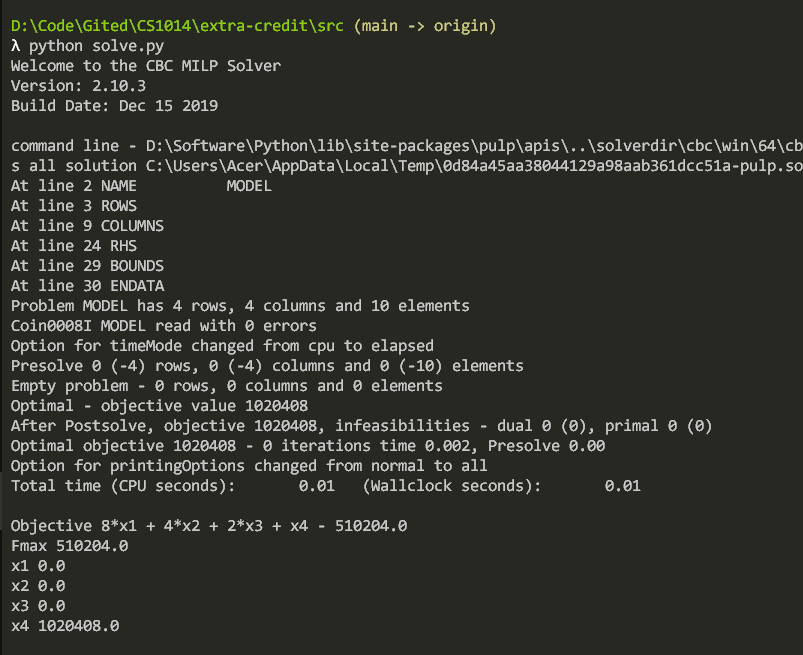
\includegraphics[scale=.85]{img/code-result.PNG}
    \caption{Kết quả kiểm thử với \texttt{pulp}}
    \label{fig:my_label}
\end{figure}
Chú ý là $8\beta_1 + 4\beta_2 + 2\beta_3 + \beta_4 = 8\times 100^0 + 4\times 100^1 + 2\times 100^2 + 100^3 = 1020408$. Tính toán tương tự với phương án tối ưu cho ra kết quả $f_{\max} = 510204$. Vậy là ta đã tính toán chính xác.

\section{Kết luận}
Bài toán Klee-Minty là một ví dụ tiêu biểu cho trường hợp tệ nhất của Phương pháp đơn hình, theo đó ta phải thực hiện tối đa $2^n - 1$ lần lặp để tìm ra phương án tối ưu. Kết hợp với ví dụ nhóm đã làm trong bài thuyết trình (i.e. chứng minh độ phức tạp của thuật toán đơn hình thuộc vào nhóm $\mathcal{O}(2^{2n})$ và đưa ra một ví dụ của bài toán Klee-Minty với $n = 3$)\cite{Nhom132022}, nhóm khẳng định các kết luận theo lí thuyết là đúng với thực tế.\\\\
Qua đó, ta phải cân nhắc một số trường hợp sử dụng Phương pháp đơn hình. Cần tính toán cẩn thận, tránh để xảy ra những sai sót không đáng có. Như một minh chứng rõ nét nhất, dù các tác giả đã sử dụng các công cụ hỗ trợ như \texttt{sympy} (tính toán symbolic) và \texttt{pulp} (kiểm chứng đáp án bài toán QHTT), nhưng vẫn tốn rất nhiều thời gian và gặp sai sót rất nhiều lần.
\cleardoublepage
\phantomsection
\addcontentsline{toc}{section}{Tài liệu}
\bibliographystyle{plain}
\bibliography{sample}
\end{document}